\documentclass[11pt]{article}
\usepackage{acl}
\usepackage{times}
\usepackage{latexsym}
\usepackage{microtype}
\usepackage{amsmath,amssymb,amsfonts}
\usepackage{algorithmic}
\usepackage{graphicx}
\usepackage{textcomp}
\usepackage{xcolor}
\usepackage{hyperref}
\usepackage{url}
\raggedbottom
% ACL titles should be in Title Case, not ALL CAPS
% center title
\title{HU at SemEval-2026 Task 6: A Hybrid Discriminative Modeling of Political Clarity and Evasion}
% Authors grouped for proper ACL formatting
\author{
  \textbf{Taha Munawar$^\dag$, Basil Ali Khan$^\dag$, Arsal Jangda$^\dag$,} \\
  \textbf{Sarfaraz Baig$^\dag$, Sandesh Kumar$^\dag$, \textnormal{and} Abdul Samad$^\dag$} \\
  $^\dag$Habib University, Dhanani School of Science \& Engineering, Pakistan \\
  \texttt{\{tm08122, bk08221, aj08514, sb08112\}@st.habib.edu.pk} \\
  \texttt{\{sandesh.kumar, abdul.samad\}@sse.habib.edu.pk}
}

\begin{document}
\maketitle

\begin{abstract}
We describe our submission to SemEval-2026 Task 6: CLARITY, which aims to classify political question--answer pairs by response clarity and evasive technique. We investigate several approaches, including long-context transformers, multiple instance learning, hierarchical multi-task models, and a natural language inference (NLI) formulation. On the development set, our best-performing NLI model achieves a macro-F1 of 0.79 for Subtask 1, while our best attention-based MIL model achieves a macro-F1 of 0.43 for Subtask 2. On the hidden evaluation set, our official submission obtains macro-F1 scores of 0.81 for Subtask 1 and 0.45 for Subtask 2. Our findings demonstrate the benefits of entailment-based modeling for clarity prediction and localized reasoning for evasion detection under limited computational resources.
\end{abstract}

\section{Introduction}
In high-stakes public discourse, particularly political interviews, the clarity of a response can be as important as its content. Speakers often employ equivocation or evasion, responding without directly answering, to deflect scrutiny or manage public perception. While such behavior has been studied extensively in political science and linguistics, its automatic detection remains a challenging Natural Language Processing (NLP) problem.

This challenge was formalized by \citet{b4} in ``I Never Said That'': A Dataset, Taxonomy and Baselines on Response Clarity Classification, which asks: \textbf{How can we automatically evaluate the clarity of a response with respect to its corresponding question?} To address this, the authors introduced a two-level hierarchical taxonomy (Fig.~\ref{fig:taxonomy}). The first level, Clarity, captures the overall directness of a response, while the second level, Evasion, identifies the specific linguistic strategy employed.

Our work addresses SemEval-2026 Task 6: CLARITY \citep{b10}, tackling both subtasks by predicting labels across this hierarchical taxonomy.

To support reproducibility, our code and experiment scripts are publicly available at \url{https://github.com/tahamunawar/semeval-task6}. The repository includes model-specific training configurations, including learning rates, batch sizes, maximum sequence lengths, warmup settings, epoch counts, loss functions, and data-processing scripts.

% The definitions for these levels are as follows: The explanation of the taxonomy label for each level is as follows:

% \textbf{Clarity Level Categories:}

% \begin{itemize}
%     \item \textbf{Clear Reply:} The information requested is explicitly provided.
%     \item \textbf{Clear Non-Reply:} The information requested is not given at all.
%     \item \textbf{Ambivalent Reply:} The information requested is given in an incomplete way.
% \end{itemize}

% \textbf{Evasion Level Categories:}

% \begin{itemize}
%     \item \textbf{Explicit:} The information requested is explicitly stated (in the requested form).
%     \item \textbf{Implicit:} The information requested is given, but without being explicitly stated (not in the expected form).
%     \item \textbf{General:} The information provided is too general or lacks the requested specificity.
%     \item \textbf{Partial:} Offers only a specific component of the requested information.
%     \item \textbf{Dodging:} Ignores the question altogether.
%     \item \textbf{Deflection:} Starts on topic but shifts the focus and makes a different point than what is asked.
%     \item \textbf{Declining to answer:} Acknowledges the question but directly or indirectly refuses to answer at the moment.
%     \item \textbf{Claims ignorance:} The answerer claims or admits not to know the answer themselves.
%     \item \textbf{Clarification:} Does not provide the requested information and instead asks for clarification.
% \end{itemize}

\begin{figure}[h!]
    \centering
    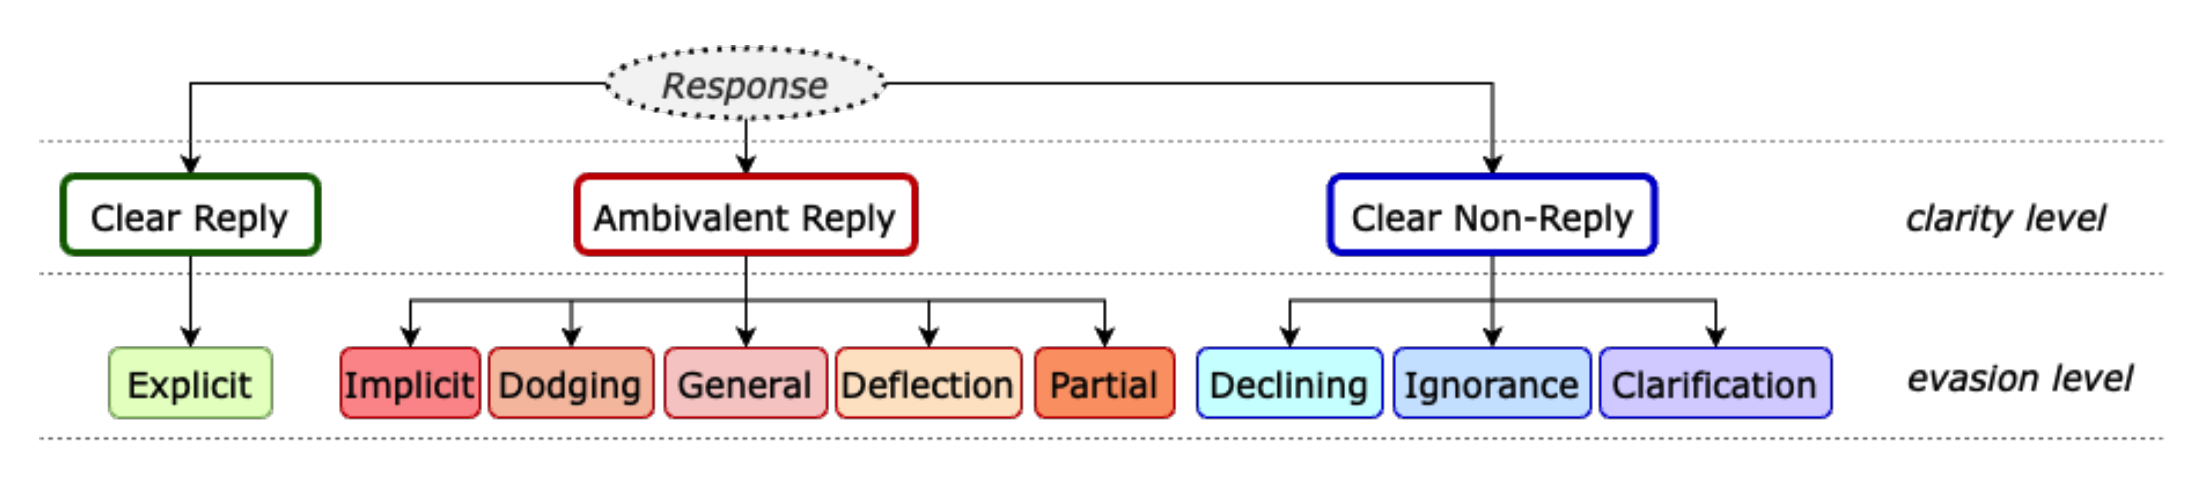
\includegraphics[width=0.9\linewidth]{taxonomy.png}
    \caption{Two-level hierarchical taxonomy for evaluating response clarity, adapted from \citet{b4}.}
    \label{fig:taxonomy}
\end{figure}

\section{Literature Review}

Research on ambiguity detection in question answering (QA) provides useful foundations for modeling political evasion. \citet{b1} show that large language models often generate coherent yet multi-faceted responses, a pattern similar to evasive political communication. Their self-consistency prompting framework combined with a lightweight Random Forest classifier outperforms larger transformer baselines, particularly in low-resource settings. Similarly, \citet{b2} introduce the AMBIENT benchmark, a linguistically annotated dataset covering lexical, syntactic, and pragmatic ambiguity, including political claims. They demonstrate that even advanced models struggle to resolve ambiguity at human-level performance, while multi-label NLI models perform more effectively, highlighting the need for domain-specific approaches. More broadly, \citet{b3} survey deep learning methods for political text analysis, emphasizing the role of contextual transformers and transfer learning in capturing nuanced political language.

Complementary work from linguistics and political science provides theoretical grounding for evasion taxonomies such as the SemEval-2026 framework. \citet{b5} define ``shifting'' as an evasive strategy in which speakers appear to address a question while subtly refocusing it, corresponding closely to the ``Deflection'' category. They identify systematic patterns such as temporal or agent shifts, abstraction changes, and non-answers. These pragmatic patterns align with categories such as Dodging, Deflection, General, and Partial replies. Additional linguistic analyses provide fine-grained examples that map to these categories, including ``non-type-conforming answers'' and divergence-minimization strategies \citep{b7}.

Unlike traditional transformers limited to 512 tokens, ModernBERT supports sequences up to 8192 tokens \citep{b8}. This addresses the risk of omitting critical evasive content due to truncation, enabling full-context modeling of lengthy political responses.

Finally, \citet{b9} introduce a self-supervised approach for assessing answer quality in political question-answer sessions by training language models to retrieve correct answers from candidate sets using only question text. Using 58,343 parliamentary exchanges from the Canadian House of Commons, they show that meaningful discourse representations can be learned without additional human annotation, suggesting that large-scale political QA corpora may provide useful domain signals for downstream question-response modeling tasks.

\section{Dataset}

Sourced from the White House (2006–2023), the dataset includes 287 presidential interview transcripts decomposed via ChatGPT-3.5 Turbo into singular QA pairs (sQAs). The final processed data comprises 3,450 training and 308 test rows, both characterized by significant class imbalance in Clarity and Evasion labels.

Due to high inter-annotator variance, Subtask 2 (Evasion) uses three ground-truth labels per test instance. Per task guidelines, a prediction is correct if it matches any of the three.

% An example of this decomposition is shown below:

% \begin{quote}
% \small % Makes the example text slightly smaller
% \textbf{Original Multi-barrelled Question:} \\
% \textit{Q. Is there a reason your press staff was unaware of that? And what did you say to the Chinese President?}

% \smallskip % Adds a small vertical space
% \textbf{Original Full Answer:} \\
% \textit{Well—and they weren't with me the entire time. Look, I made it clear that I thought that China had an obligation to be more forthcoming on exactly what the source of the virus was and where it came from.Yes.}

% \smallskip

% \textbf{Resulting sQA Pair 1:}
% \begin{itemize}
%     \item \textbf{Sub-question:} \textit{Is there a reason your press staff was unaware of that?}
%     \item \textbf{Full Answer:} \textit{Well—and they weren't with me the entire time. Look, I made it clear that I thought that China had an obligation to be more forthcoming on exactly what the source of the virus was and where it came from.Yes.}
% \end{itemize}

% \textbf{Resulting sQA Pair 2:}
% \begin{itemize}
%     \item \textbf{Sub-question:} \textit{What did you say to the Chinese President?}
%     \item \textbf{Full Answer:} \textit{Well—and they weren't with me the entire time. Look, I made it clear that I thought that China had an obligation to be more forthcoming on exactly what the source of the virus was and where it came from.Yes.}
% \end{itemize}
% \end{quote}

% The resulting dataset had two splits: a training set with 3,450 rows and a test set with 308 rows, with the important columns being ``interview\_question'', ``interview\_answer'', ``question'', ``clarity\_label'', and ``evasion\_label''.

% We noted that the evasion\_label column was empty in the test set. The researchers clarified this was intentional. They found that annotators had disagreements (high variance) when assigning these labels, so they decided against using a single ``ground truth'' label.

% Instead, the test set provides the individual labels from three annotators in the ``annotator1'', ``annotator2'', and ``annotator3'' columns. For evasion level prediction, a model's prediction is considered correct if it matches any of these three labels.

% Moreover, the dataset exhibited significant class imbalance in both clarity and evasion labels, as shown in the figures below.

% \begin{figure}[h!]
%     \centering
%     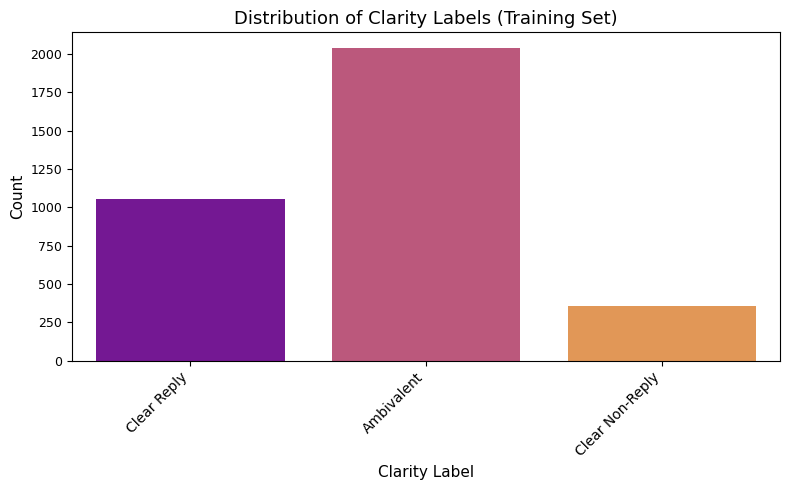
\includegraphics[width=0.9\linewidth]{clarity_count.png}
%     \caption{Distribution of clarity level labels in the dataset.}
%     \label{fig:clarity_count}
% \end{figure}

% \begin{figure}[h!]
%     \centering
%     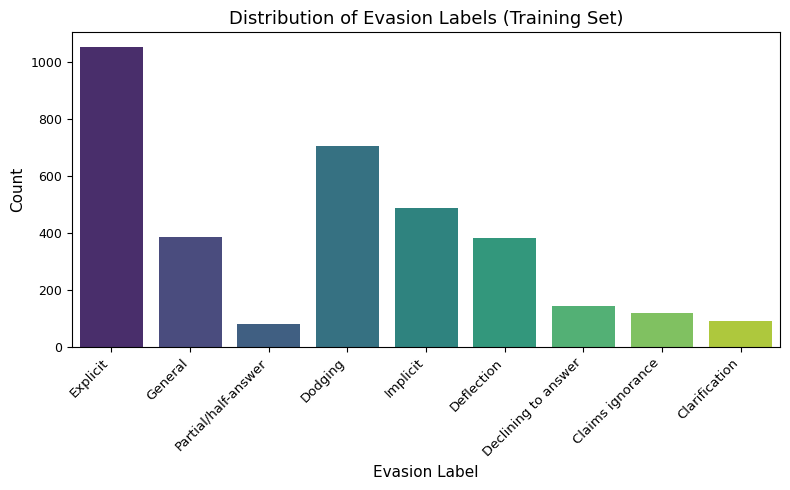
\includegraphics[width=0.9\linewidth]{evasion_count.png}
%     \caption{Distribution of evasion level labels in the dataset.}
%     \label{fig:evasion_count}
% \end{figure}


\section{Methodology}

We propose six architectural approaches for this task and explore data augmentation strategies to mitigate class imbalance.

\subsection{Task Formulation and Evaluation}
Given a question $Q$ and an answer $A$, the objective is to predict the high-level clarity label for Subtask 1 and the fine-grained evasion label for Subtask 2. We use macro-F1 as the primary evaluation metric.

For Subtask 1, each instance has a single gold clarity label. For Subtask 2, each instance has three annotator-provided evasion labels, which are treated as a set of acceptable gold labels $G_i$. A prediction $\hat{y}_i$ is considered correct for class $y$ if $\hat{y}_i = y$ and $y \in G_i$. Following the official scorer for the shared task \citep{b10}, per-class precision, recall, and F1 are computed using this set-valued gold criterion, and the final score is the unweighted mean across evasion classes:
\[
F1_{\text{macro}} = \frac{1}{|\mathcal{Y}|}\sum_{y \in \mathcal{Y}} F1_y.
\]
To mitigate class imbalance, we experimented with Focal Loss, Weighted Cross-Entropy, and Dice Loss across architectural variants.

\subsection{Direct Classification (ModernBERT)}
To preserve the full context of sQA pairs, we fine-tune \texttt{ModernBERT-base} and \texttt{large}, leveraging their native 8192-token sequence length to capture the complete interaction within a single classification head \citep{b8}, without having to truncate long political responses.

\subsection{Multiple Instance Learning (MIL)}
To address the input length constraint without relying solely on newer architectures, we implemented a Multiple Instance Learning (MIL) framework with Attention Pooling. This approach is particularly relevant for Subtask 2, where the specific ``evasion technique" (e.g., a deflection) may occur in a small segment of a long answer.

We split the long answers into overlapping segments, or instances, such that for an input pair $(Q, A)$, the answer $A$ forms a bag of instances $\mathcal{I} = \{I_1, I_2, \dots, I_k\}$.

\begin{itemize}
    \item \textbf{Input Formatting:} Each instance $I_i$ was constructed by concatenating the full question $Q$ and an answer segment $A_{\text{segment}}$ using the standard BERT format: $I_i = [\texttt{CLS}] \ Q \ [\texttt{SEP}] \ A_{\text{segment}} \ [\texttt{SEP}]$.
    \item \textbf{Chunking Parameters:} Maximum length $256$ tokens with $160$-token stride, limiting instances to $k \le 16$.
    \item \textbf{Attention Pooling:} Each instance is encoded independently (frozen encoder) to obtain $\mathbf{h}_i$ from the final $[\texttt{CLS}]$ state, followed by learnable attention weights $\alpha_i$ to produce $\mathbf{c} = \sum_{i=1}^{k} \alpha_i \mathbf{h}_i$ for classification.

\end{itemize}

We experimented with multiple encoders, including BERT \citep{devlin2019bert}, RoBERTa \citep{liu2019roberta}, DeBERTa \citep{he2021deberta}, and ALBERT \citep{lan2020albert}.

\subsection{Natural Language Inference (NLI)}
For Subtask 1 (Clarity Prediction), we hypothesized that the concept of ``clarity" is fundamentally related to logical entailment. We effectively reframed the classification task into a three-way Natural Language Inference (NLI) problem. For every Question-Answer pair $(Q, A)$, we constructed an NLI input consisting of a Premise and a Hypothesis:

\begin{itemize}
    \item \textbf{Premise ($P$):} The politician's full answer $\{A\}$.
    \item \textbf{Hypothesis ($H$):} ``The speaker explicitly answers the Question: $\{Q\}$."
\end{itemize}

We used the specialized NLI model \texttt{MoritzLaurer/\allowbreak DeBERTa-v3-large-\allowbreak mnli-fever-anli-ling-wanli}, pre-trained on multiple NLI and factual consistency tasks. NLI has been widely used for modeling entailment relationships between premise--hypothesis pairs \citep{bowman2015large}. While \citet{b4} noted that traditional encoder-only classifiers are often constrained by 512-token inputs, we set the maximum sequence length to 2048 tokens for this model. This allowed substantially more of the answer context to be retained, although it remained bounded by available GPU memory. We treat this as an implementation choice rather than an architectural guarantee, since the model was not originally introduced as a long-context encoder.

We map NLI labels to clarity categories as follows: \textbf{Entailment} $\rightarrow$ \textbf{Clear Reply}, \textbf{Contradiction} $\rightarrow$ \textbf{Clear Non-Reply}, and \textbf{Neutral} $\rightarrow$ \textbf{Ambivalent Reply}.

\subsubsection{Adversarial Weight Perturbation (AWP)}
We applied AWP \citep{wu2020adversarial} to improve robustness by encouraging flatter minima. During training, weights $\theta$ are perturbed along the gradient direction:
\begin{equation*}
\theta_{adv} = \theta + \epsilon \frac{\nabla_\theta \mathcal{L}(\theta)}{\|\nabla_\theta \mathcal{L}(\theta)\|_2}
\end{equation*}
with $\epsilon = 10^{-3}$ starting from the second epoch.


\subsubsection{Hybrid Probability Calibration and Blending}
To reconcile biases between different calibration methods, we implemented a Weighted Probability Blend (Soft Voting). We utilized Isotonic Regression ($P_{iso}$) to act as a conservative estimator and Temperature Scaling ($P_{ts}$) to serve as a liberal estimator by softening probability distributions. The final probability distribution $P_{final}$ is the weighted average of the two calibrated distributions:
$$P_{final} = w_{iso} P_{iso} + (1 - w_{iso}) P_{ts}$$

This NLI formulation was effective for Subtask 1 because its three outputs aligned directly with the clarity labels. We did not extend it to Subtask 2 in the final system because the nine evasion categories do not admit the same direct one-to-one mapping from entailment, contradiction, and neutral. A possible extension would require testing multiple label-specific hypotheses per instance and then designing an aggregation rule over the resulting NLI scores. We considered this design informally, but running it properly was computationally expensive and difficult to validate under our resource constraints.

\subsection{Generative Approach}
We explored the capabilities of generative LLMs by fine-tuning the \texttt{Llama-3.2-3B} instruct model \citep{meta2024llama32}. Due to computational constraints, we used 4-bit quantization with QLoRA \citep{dettmers2023qlora}. The inputs consisted of each question--answer pair provided directly to the model, and it was prompted to generate the classification label. For training stability and efficiency, we applied LoRA \citep{hu2021lora} with an \textbf{r} value of \textbf{16} and an \textbf{alpha} of \textbf{32}.

We report this approach only for Subtask 1 in our main results because preliminary Subtask 2 experiments were less reliable than the discriminative MIL setup under the same compute constraints. We therefore did not use the generative model for the final Subtask 2 submission.

\subsection{Multi-Task Hierarchical Gating (MTL)}
We implemented a Multi-Task Learning (MTL) architecture using ModernBERT-large to jointly optimize Clarity and Evasion labels. The model utilizes a hierarchical gating mechanism where the Clarity Head first computes the probability distribution $P(c|h)$. This distribution is projected into a gating vector $g = \sigma(W_g P(c|h) + b_g)$, which modulates the shared representation via $h_{gated} = h \odot g$ to isolate features relevant to the predicted clarity level. To enforce taxonomic logic, we introduced a Consistency Loss, $\mathcal{L}_{cons} = \sum_{i} \text{softplus}(P(e_i) - P(c_{M(e_i)}))$, which penalizes child label probabilities that exceed those of their parent. The final objective is a weighted sum: $\mathcal{L}_{total} = \alpha \mathcal{L}_{evasion} + \beta \mathcal{L}_{clarity} + \gamma \mathcal{L}_{cons}$.

\subsection{Hierarchy-Aware Global Model (HiAGM)}
To capture taxonomic dependencies, we implemented a Hierarchy-Aware Global Model (HiAGM) \citep{zhou2020hierarchy} that treats labels as a directed graph $\mathcal{G} = (\mathcal{V}, \mathcal{E})$. We utilize a single-layer Graph Convolutional Network (GCN) to learn hierarchy-aware embeddings, $W_{labels} = \text{ReLU}(\tilde{A} \cdot E \cdot W_g)$, allowing feature propagation from parent clarity labels to child evasion techniques. Using ModernBERT-base as a text encoder (1024-token sequence), final logits are computed via dot-product compatibility: $\text{Logits} = h \cdot (W_{labels})^\top$. The model is optimized via Focal Loss ($\gamma=3.0$) with class weights. To ensure 100\% hierarchical consistency, Subtask 1 labels are deterministically inferred post-hoc from the predicted Subtask 2 leaf nodes.

\subsection{Data Augmentation}
We experimented with several augmentation strategies to improve robustness:

\begin{itemize}
    \item \textbf{Random Word Deletion:} \texttt{nlpaug}-based deletion applied to answer text, generating augmented samples equal to 25\% of the original data per clarity class.
    \item \textbf{Oversampling:} Weighted random sampling using inverse class frequency to mitigate imbalance without explicit duplication.
    \item \textbf{Contextual Word Replacement:} Masked language model–based substitutions using \texttt{nlpaug} (BERT).
    \item \textbf{Back-Translation:} English $\rightarrow$ German $\rightarrow$ English via Gemini 2.5 Flash, applied selectively to misclassified samples identified through 5-fold cross-validation.
    \item \textbf{Few-Shot Synthetic Generation:} Gemini 2.5 Flash prompted with minority-class examples to generate additional question–answer pairs.
\end{itemize}

These techniques were applied across both subtasks to address class imbalance.

% It is important to note, however, that after extensive experimentation, these augmentation techniques did not result in a net increase in F1 scores for our tasks. As a result, the final models presented in Section 5 rely solely on the original dataset.

\section{Results and Discussion}

\subsection{Model Selection and Internal Benchmarking}
Table \ref{tab:results} compares our best architectural approaches on the \textbf{development set}, against the baseline benchmarks established by the task organizers \citep{b4}.

\begin{table}[h]
\centering
\small
\begin{tabular}{lcc}
\hline
\textbf{Model} & \textbf{T1} & \textbf{T2} \\
\hline
Baseline: Llama-2-70B & 0.68 & 0.51 \\
\hline
Gen: Llama-3.2-3B & 0.57 & - \\
Direct: ModernBERT-L & 0.69 & 0.38 \\
\textbf{MIL: DeBERTa-v3-B} & 0.65 & \textbf{0.43} \\
\textbf{NLI: DeBERTa-v3-L} & \textbf{0.79} & - \\
MTL: ModernBERT-L & 0.64 & 0.40 \\
HiAGM: ModernBERT-L & 0.52 & 0.40 \\
\hline
\end{tabular}
\caption{Comparison with the organizers' development-set baseline. T1 = Subtask 1, T2 = Subtask 2.}
\label{tab:results}
\end{table}


\subsubsection{Final Evaluation Results}
After selecting the best-performing models based on development-set performance, we evaluated them on the hidden evaluation set. Our official SemEval-2026 Task 6 submission achieved a final leaderboard rank of \textbf{8} for Subtask 1 and \textbf{17} for Subtask 2 in the shared task \citep{b10}. The corresponding macro-F1 scores are shown in Table~\ref{tab:final}.

\begin{table}[h]
\centering
\small
\begin{tabular}{llcc}
\hline
\textbf{Task} & \textbf{Model} & \textbf{Dev} & \textbf{Eval} \\
\hline
Subtask 1 & Llama-2-70B baseline & 0.68 & 0.82 \\
Subtask 1 & NLI: DeBERTa-v3-L & \textbf{0.79} & 0.81 \\
\hline
Subtask 2 & Llama-2-70B baseline & 0.51 & 0.57 \\
Subtask 2 & DeBERTa-v3-B + MIL & 0.43 & 0.45 \\
\hline
\end{tabular}
\caption{Development and hidden evaluation performance. Baseline scores are shown separately for the development and hidden evaluation splits to avoid cross-split comparison.}\label{tab:final}
\end{table}

\subsection{Comparison with Benchmark and Shared-Task Systems}
A key finding of our work is the efficiency--performance trade-off relative to the organizers' Llama-2-70B baseline. While the baseline uses a 70B-parameter generative model, our best Subtask 1 model uses DeBERTa-v3-large, with roughly 400M parameters. On the development set, our NLI formulation improves Subtask 1 macro-F1 from 0.68 to 0.79; on the hidden evaluation set, it remains competitive with the baseline (0.81 vs. 0.82), though not superior.

The broader shared-task results further contextualize this trade-off. The strongest Subtask 1 systems relied mainly on LLM prompting, multi-stage reasoning, and hierarchical mappings, with the top system reaching 0.89 macro-F1 \citep{b10}. Our result suggests that a smaller NLI-based encoder can remain competitive when clarity prediction is framed as entailment. For Subtask 2, however, the baseline and top shared-task systems remain substantially stronger, indicating that fine-grained evasion detection benefits from taxonomy-aware routing, constrained label spaces, and LLM-based verification beyond segment-level MIL.

\subsection{Performance Analysis}

\subsubsection{Context vs. Segmentation in Evasion}
For Subtask 2, the Multiple Instance Learning (MIL) approach outperformed ModernBERT (0.43 vs. 0.38). While ModernBERT captures the entire context (8192 tokens), the ``evasion" label is often localized. The global pooling of ModernBERT may dilute these specific signals. In contrast, the Attention Pooling mechanism in MIL explicitly assigns high weights to the most discriminative segments of the answer, effectively isolating the evasion tactic.

\begin{table}[h]
\centering
\scriptsize
\begin{tabular}{lcccc}
\hline
\textbf{Class} & \textbf{Support} & \textbf{Prec.} & \textbf{Rec.} & \textbf{F1} \\
\hline
Claims ignorance & 14 & 0.83 & 0.71 & 0.77 \\
Clarification & 4 & 0.67 & 0.50 & 0.57 \\
Declining to answer & 13 & 0.29 & 0.54 & 0.38 \\
Deflection & 29 & 0.31 & 0.17 & 0.22 \\
Dodging & 72 & 0.54 & 0.29 & 0.38 \\
Explicit & 88 & 0.77 & 0.23 & 0.35 \\
General & 92 & 0.56 & 0.38 & 0.45 \\
Implicit & 82 & 0.41 & 0.57 & 0.48 \\
Partial/half-answer & 12 & 0.27 & 0.25 & 0.26 \\
\hline
\end{tabular}
\caption{Per-class development-set performance of the MIL model for Subtask 2. Support is computed as TP+FN under the official set-valued gold-label criterion.}
\label{tab:subtask2_per_class}
\end{table}

The MIL model performs best on relatively explicit refusal-like categories such as \textit{Claims ignorance} and \textit{Clarification}, while performance is weakest for more pragmatically subtle categories such as \textit{Deflection}, \textit{Dodging}, and \textit{Partial/half-answer}. This broadly aligns with the evasion-level annotation difficulty reported by \citet{b4}, where annotators showed high disagreement among closely related categories such as \textit{General}, \textit{Implicit}, \textit{Deflection}, and \textit{Dodging}. In particular, \citet{b4} report low pairwise agreement for \textit{General} vs. \textit{Implicit} ($\kappa=0.43$), \textit{General} vs. \textit{Deflection} ($\kappa=0.56$), \textit{General} vs. \textit{Dodging} ($\kappa=0.57$), and \textit{Dodging} vs. \textit{Deflection} ($\kappa=0.62$). Since we do not compute a model-level confusion matrix, we interpret this only as supporting evidence that several low-F1 categories correspond to inherently difficult evasion distinctions.

\subsubsection{The Trade-off of Hierarchical Constraints}
While the Multi-Task Hierarchical Gating (MTL) and Hierarchy-Aware Global Model (HiAGM) were designed to explicitly model the taxonomic dependencies described in Sections 4.6 and 4.7, they achieved lower macro-F1 scores (0.64 and 0.52 respectively) on Subtask 1 compared to the NLI approach. We observe that the Hierarchical Consistency Loss ($\mathcal{L}_{cons}$) and the post-hoc deterministic inference used in HiAGM may have been overly restrictive. By forcing the model to strictly adhere to the parent-child relationship, we likely introduced a "bottleneck" where errors in fine-grained evasion detection (Subtask 2) propagated upward, penalizing the clarity prediction (Subtask 1). In contrast, the NLI model's flexibility to treat clarity as a logical entailment problem allowed for better generalization across varied presidential rhetorical styles.

\subsubsection{The Generative Lag}
Our generative approach (\texttt{Llama-3.2-3B}) underperformed, achieving only 0.57 F1. We observed early overfitting, with performance dropping from 0.57 to 0.50 between epochs. This reinforces our finding that without the massive scale of the researchers' $70\text{B}$ model, generative decoding is less stable than discriminative classification for this task.

\subsubsection{Inefficacy of Augmentation}
The data augmentation strategies in Section 4.8 did not improve macro-F1 for either Subtask 1 or 2.

We attribute this to the \textit{fragility of political nuance}. Political evasion depends on subtle rhetorical cues (e.g., ``shifting'' or ``flouting Gricean Maxims''), making class boundaries highly sensitive to perturbations. This is consistent with \citet{b4}, who reported low inter-annotator agreement ($\kappa = 0.48$) and difficulty distinguishing semantically proximate categories such as \textit{General} and \textit{Implicit}. Such inherent ambiguity likely caused both lexical augmentation and LLM-generated data to introduce noise rather than useful diversity, explaining the lack of performance gains.

We also experimented with intermediate domain pre-training on external political question–answer data (as described in Section~2). However, this did not yield measurable improvements, likely because the source domain (parliamentary proceedings) differs substantially from the target domain (presidential interviews), limiting transfer effectiveness given the small downstream dataset.

\begin{table}[h]
\centering
\small
\begin{tabular}{llc}
\hline
\textbf{Task} & \textbf{Augmentation Strategy} & \textbf{Macro-F1} \\
\hline
Subtask 1 & \textit{None (Best Model)} & \textbf{0.79} \\
& Random Word Deletion & 0.72 \\
& Weighted Oversampling & 0.69 \\
& Contextual Word Replacement & 0.73 \\
& Back-Translation & 0.74 \\
& Few-Shot Synthetic Generation & 0.70 \\
\hline
Subtask 2 & \textit{None (Best Model)} & \textbf{0.43} \\
& Random Word Deletion & 0.41 \\
& Weighted Oversampling & 0.42 \\
& Contextual Word Replacement & 0.39 \\
& Back-Translation& 0.40 \\
& Few-Shot Synthetic Generation & 0.43 \\
\hline
\end{tabular}
\caption{Detailed impact of five data augmentation techniques on top-performing models for Subtask 1 and Subtask 2.}
\label{tab:augmentation_full_results}
\end{table}

\subsubsection{NLI Calibration and Error Analysis}
Initial experiments revealed significant semantic overlap between the \textit{Clear Reply} and \textit{Ambivalent} classes, leading to a performance bottleneck. This aligns with \citet{b4}, who reported that annotators struggled most to distinguish between the parent categories \textit{Clear Reply} and \textit{Ambivalent} in the clarity dimension, with inter-annotator agreement dropping to $\kappa = 0.65$, compared to much higher agreement for other high-level distinctions. The introduction of AWP proved vital, seeking a flatter loss landscape that improved the macro-F1 from 0.70 to 0.74 by enhancing model robustness against varied political phrasing. Building on this, our hybrid post-training probability calibration further decoupled the remaining semantic overlap, resulting in our final development-set macro-F1 score of 0.79. Our analysis showed that the distinct calibration methods yielded specific performance biases: Isotonic Regression ($P_{iso}$) provided high precision (0.84) for clear replies, while Temperature Scaling ($P_{ts}$) recovered recall (0.78). Through a grid search on the validation set, we determined the optimal temperature to be $T = 1.23$ and the optimal weighting factor to be $w_{iso} = 0.59$. 

\section{Limitations}
A primary challenge in our experimentation was the significant computational disparity between our infrastructure and the task's 70B-parameter baseline. Our generative fine-tuning was restricted by Kaggle and Google Colab runtime limits, where the 8-hour-per-epoch training cycle frequently triggered platform timeouts and session disconnections. These compute constraints prevented us from performing exhaustive hyperparameter tuning or completing longer training runs, which likely contributed to the ``generative lag'' observed in our results.

A further limitation is that most results are based on single development-set runs rather than multi-seed averages. This is especially relevant for Subtask 2, where several evasion categories have low support and may therefore be sensitive to random initialization and sampling effects. In addition, although the final NLI system used a validation-selected calibration blend with $w_{iso}=0.59$, we did not perform an extensive sensitivity analysis of this weight. Future work should evaluate whether the calibration gains remain stable across seeds and whether they improve all clarity classes uniformly or mainly benefit the difficult \textit{Clear Reply}--\textit{Ambivalent Reply} boundary.

% In future work, we plan to use Synthetic Data Generation as an augmentation strategy. We will prompt a large instruction-tuned model (e.g., Gemini 2.5 Flash API or GPT-5-mini) using a few-shot setup. For each of the 3 Clarity Level classes and 9 Evasion Level classes, we will provide the model with \textbf{5} manually selected question--answer examples representing that class. The model will then be instructed to generate new question--answer pairs that strictly follow the target label, allowing us to create high-quality synthetic samples to expand our training dataset.

% We also intend to explore smaller open-source generative LLMs (e.g., Qwen, Mistral) that have shown performance competitive with or exceeding larger models, to assess whether the strategy of using generative LLMs to predict Evasion labels is still feasible or not.

\pagebreak

\bibliography{custom} % This points to custom.bib
\end{document}